\chapter{Tutorial HelloWorld for Java}

\section{Scope}

In this tutorial you will build your first very simple eTrice model. The goal is to learn the work flow of eTrice and to understand a few basic features of ROOM. You will perform the following steps:

\begin{enumerate}
\item create a new model from scratch
\item add a very simple state machine to an actor
\item generate the source code
\item run the model
\item open the message sequence chart
\end{enumerate}

Make sure that you have set up the workspace as described in \textit{Setting up the workspace}.

\section{Create a new model from scratch}

The easiest way to create a new eTrice Project is to use the eclipse project wizard. From the eclipse file menu select \textbf{File->New->Project} and create a new eTrice project and name it \textbf{HelloWorld}.

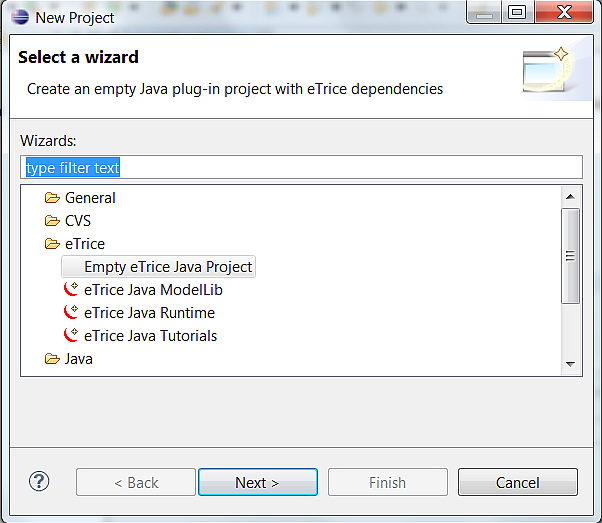
\includegraphics[width=\linewidth]{images/015-HelloWorld10.png}
% !images/015-HelloWorld10.png!

The wizard creates everything that is needed to create, build and run an eTrice model. The resulting project should look like this:

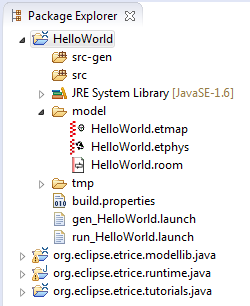
\includegraphics{images/015-HelloWorld11.png}
% !images/015-HelloWorld11.png!

Within the model directory the model file \textit{HelloWorld.room} was created. Open the \textit{HelloWorld.room} file and delete the contents of the file. Open the content assist with Ctrl+Space and select \textit{model skeleton}.

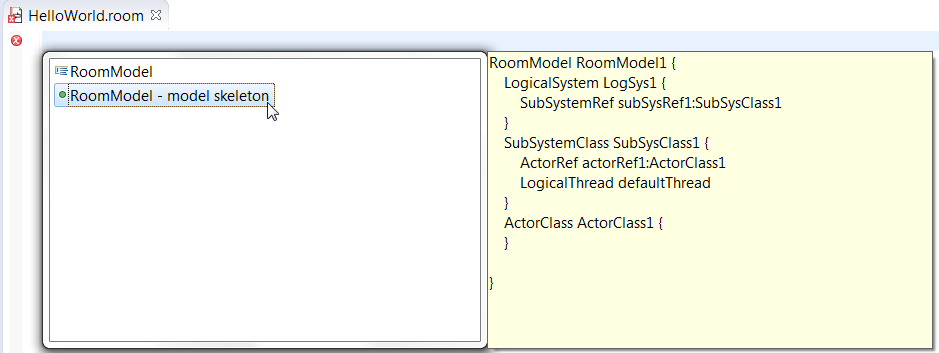
\includegraphics[width=\linewidth]{images/015-HelloWorld12.png}
% !images/015-HelloWorld12.png!   

Edit the template variables by typing the new names and jumping with Tab from name to name.

The resulting model code should look like this:

\begin{verbatim}
RoomModel HelloWorld {

    LogicalSystem System_HelloWorld {
        SubSystemRef subsystem : SubSystem_HelloWorld
    }

    SubSystemClass SubSystem_HelloWorld {
        ActorRef application : HelloWorldTop
    }

    ActorClass HelloWorldTop {
    }
} 
\end{verbatim}

The goal of eTrice is to describe distributed systems on a logical level. In the current version not all elements will be used. But as prerequisite for further versions the following elements can be defined:
\begin{itemize}
\item the \textit{LogicalSystem} (currently optional)
\item at least one \textit{SubSystemClass} (mandatory)
\item at least one \textit{ActorClass} (mandatory)
\end{itemize}

The \textit{LogicalSystem} represents the complete distributed system and contains at least one \textit{SubSystemRef}. The \textit{SubSystemClass} represents an address space and contains at least one \textit{ActorRef}. The \textit{ActorClass} is the building block of which an application will be built of. It is in general a good idea to define a top level actor that can be used as reference within the subsystem.

The outline view of the textual ROOM editor shows the main modeling elements in an easy to navigate tree.

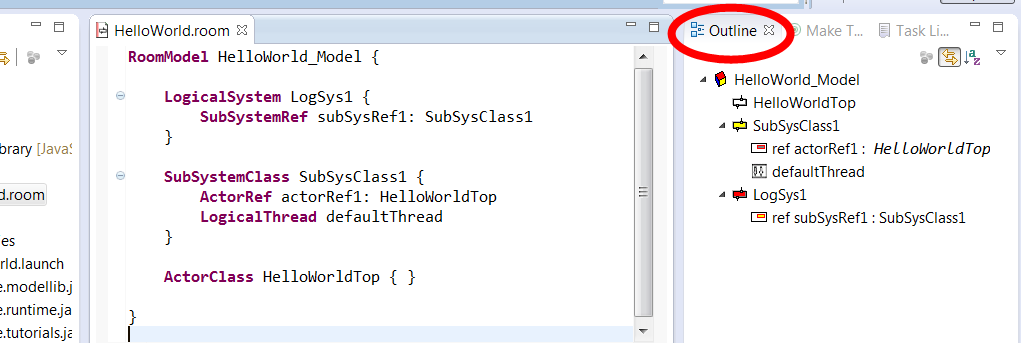
\includegraphics[width=\linewidth]{images/015-HelloWorld02.png}
% !images/015-HelloWorld02.png!


\section{Create a state machine}

We will implement the Hello World code on the initial transition of the \textit{HelloWorldTop} actor. Therefore open the state machine editor by right clicking the \textit{HelloWorldTop} actor in the outline view and select \textit{Edit Behavior}.

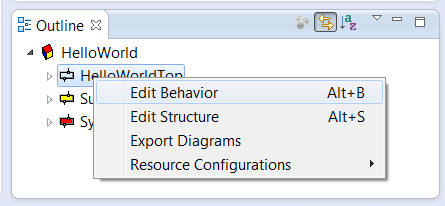
\includegraphics{images/015-HelloWorld03.png}
% !images/015-HelloWorld03.png!

The state machine editor will be opened. Drag and drop an \textit{Initial Point} from the tool box to the diagram into the top level state. Drag and drop a \textit{State} from the tool box to the diagram. Confirm the dialogue with \textit{ok}. Select the \textit{Transition} in the tool box and draw the transition from the \textit{Initial Point} to the State. Open the transition dialogue by double clicking the transition arrow and fill in the action code.

\begin{verbatim}
	System.out.println("Hello World !");
\end{verbatim}
 
The result should look like this:

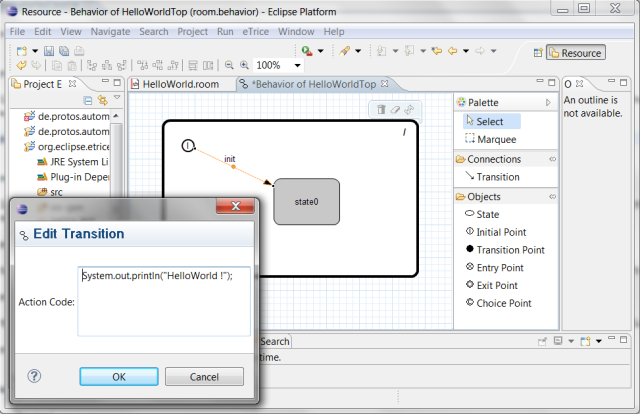
\includegraphics[width=\linewidth]{images/015-HelloWorld04.png}
% !images/015-HelloWorld04.png!

Save the diagram and inspect the model file. Note that the textual representation was created after saving the diagram.

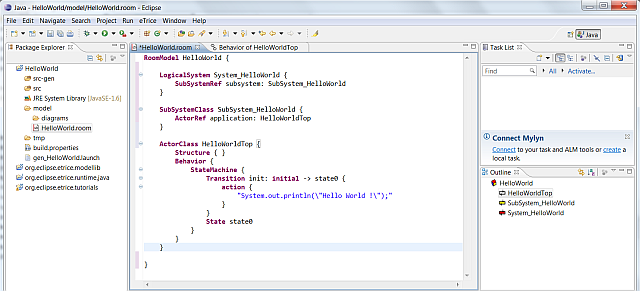
\includegraphics[width=\linewidth]{images/015-HelloWorld05.png}
% !images/015-HelloWorld05.png!


\section{Build and run the model}

Now the model is finished and source code can be generated. The project wizard has created a launch configuration that is responsible for generating the source code. From \textit{HelloWorld/} right click \textbf{gen\_HelloWorld.launch} and run it as gen\_HelloWorld. All model files in the model directory will be generated.

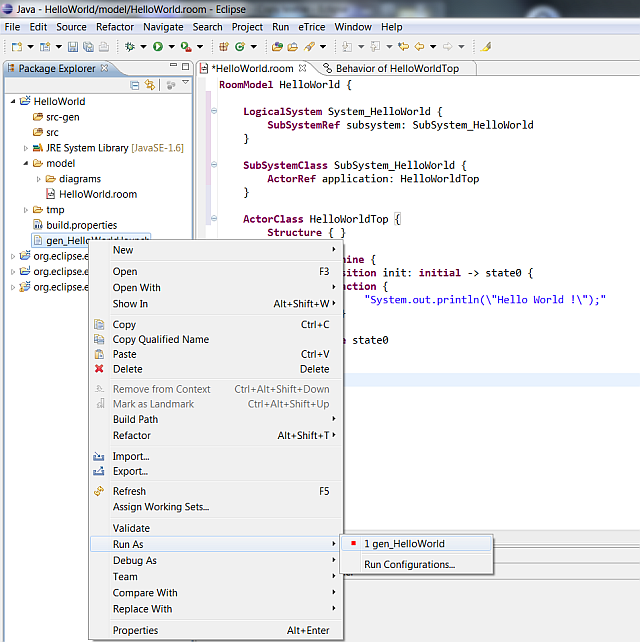
\includegraphics[width=\linewidth]{images/015-HelloWorld06.png}
% !images/015-HelloWorld06.png!

The code will be generated to the src-gen directory. The main function will be contained in \textbf{SubSystem\_HelloWorldRunner.java}. Select this file and run it as Java application.

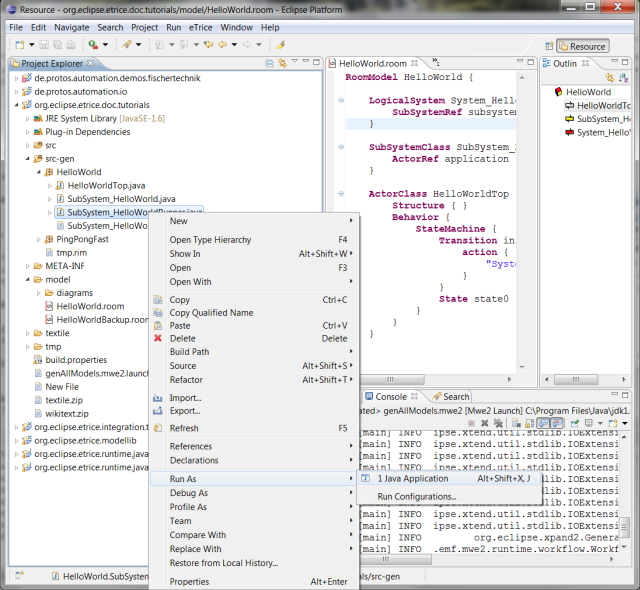
\includegraphics{images/015-HelloWorld07.png}
% !images/015-HelloWorld07.png!


The Hello World application starts and the string will be printed on the console window. To stop the application the user must type \textbf{quit} in the console window.

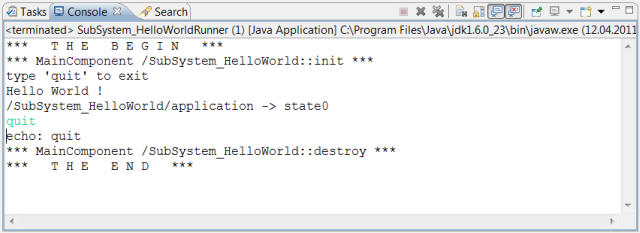
\includegraphics[width=\linewidth]{images/015-HelloWorld08.png}
% !images/015-HelloWorld08.png!

\section{Open the Message Sequence Chart}

During runtime the application produced a MSC and wrote it to a file. Open HelloWorld/tmp/log/SubSystem\_HelloWorld\_Async.seq using Trace2UML (it is open source and can be obtained from  http://trace2uml.tigris.org/). You should see something like this:

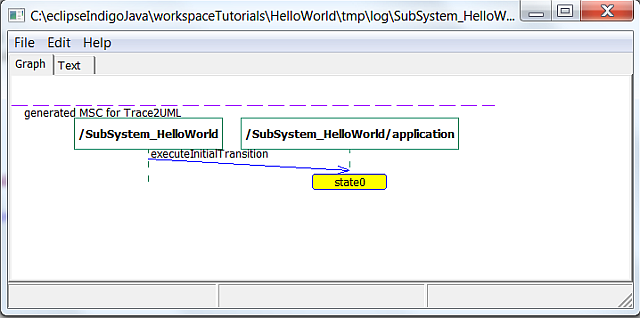
\includegraphics[width=\linewidth]{images/015-HelloWorld09.png}
% !images/015-HelloWorld09.png!


\section{Summary}

Now you have generated your first eTrice model from scratch. You can switch between diagram editor and model (.room file) and you can see what will be generated during editing and saving the diagram files. 
You should take a look at the generated source files to understand how the state machine is generated and the life cycle of the application. The next tutorials will deal with more complex hierarchies in structure and behavior.
